\chapter{Fungovanie stránky}
\section{Súbory tvoriace stránku}

Všetky stránky a podstránky sú graficky ovládané pomocou 6 súborov .css ktoré sú logicky usporiadané podľa celkov kódu. Celá stránka sa skladá z 18 podstránok a 2 databáz.

\subsection{domovská stránka}
\vspace{0.5cm}
\textbf{Začiatočná deklarácia stránky je na každej stránke rovnaká, ďalej ju teda nebudeme pripájať.}
\vspace{0.5cm}
\begin{lstlisting}
<!DOCTYPE HTML>
<head>
<meta http-equiv="Content-Type" content="Stranka slavky fratricovej" charset="UTF-8">
<meta name="Author" content="Peter Tibensky, STU">
<meta http-equiv="content-language" content="sk">
<link rel="stylesheet" href="css/default.css">
<link rel="stylesheet" href="css/layout.css">
<link rel="stylesheet" href="css/media-queries.css">
<link rel="stylesheet" type="text/css" href="style.css">
<title>SF</title>
<link rel="shortcut icon" href="favicon.png" >
</head>
\end{lstlisting}
\vspace{0.5cm}
\textbf{Kód headeru každej stránky je rovnaký, ďalej ho teda nebudeme pripájať. V headeri sú určené buttony, ich prepojenia a taktiež úvodné logo ktoré slúži ako button.}
\vspace{0.5cm}
\begin{lstlisting}
<body>

<?php
require_once "config.php";
?>
<button class="open-button pointer" onclick="openForm()"></button>
<div class="form-popup " id="myForm">
<a href='login.php' class="button10"></a>
</div>
<script>
function openForm() {
document.getElementById("myForm").style.display = "block";
}
function closeForm() {
document.getElementById("myForm").style.display = "none";
}
</script>
<div class="logo center">
<a href="index.php"><img src="favicon.png" alt='Home' ></a>
</div>
<div class="topnav">
<div class="flex-parent jc-center ">
<a href='indexx.php' class="button button1 font">texty</a>
<a href='foto.php' class="button button1 font">foto</a>
<a href='portfolko.php' class="button button1 font">portfolko</a>
</div>
</div>

\end{lstlisting}
\vspace{0.5cm}
\textbf{Vystrihnutá časť lorem ipsum, pokiaľ na stránke nevymyslíme iný úvodný text.}
\vspace{0.5cm}
\begin{lstlisting}

<div class="popis font">
<p>
Lorem ipsum...
</p>
</div>
<div class="popis font">
<p>
Curabitur molestie...
</p>
</div>

\end{lstlisting}
\vspace{0.5cm}
\textbf{Footer, v ktorom sa nachádzajú linky na sociálne siete a email. }
\vspace{0.5cm}
\begin{lstlisting}
<hr style="height:2px;border-width:0;color: #FFD658 ;background-color: #FFD658">
<div class="flex-parent jc-center ">
<div class=" column font ">
<img src="in.png" alt="linkedin" style="width:4.5%">
<a class="five" href="https://www.linkedin.com/in/slavka-fratricova" target="_blank">www.linkedin.com/in/slavka-fratricova</a>
</div>
<div class=" column font">
<img src="email.png" alt="email" style="width:5.8%">
<a href = "mailto: slavka.fratricova@gmail.com">slavka.fratricova@gmail.com</a>
</div>
</div>
</body>
\end{lstlisting}

\subsection{texty}
\vspace{0.5cm}
\textbf{Pripojenie ku databáze a získanie údajov potrebných pre vypísanie textov.}
\vspace{0.5cm}
\begin{lstlisting}
<?php
include_once('resources/init.php');
//$posts = (isset($_GET['id'])) ? get_posts($_GET['id']) : get_posts();
$posts = get_posts((isset($_GET['id']))? $_GET['id'] : null);
?>


\end{lstlisting}
\vspace{0.5cm}
\textbf{Vypísanie jednotlivých textov.}
\vspace{0.5cm}
\begin{lstlisting}
<div id="content-wrap">
<div class="row">
<article class="entry">
<?php
foreach($posts as $post){
?>
<header class="entry-header">
<h2><a href='indexx.php?id=<?php echo $post['post_id']; ?>' ><?php echo $post['title']; ?></a></h2>						
<div class="entry-meta">
<ul>
<li> <?php echo date('d-m-y h:i:s',strtotime($post['date_posted'])); ?></li>
</ul>
</div>
</header>
<?php}
?>
<div class="entry-content font">
<p><?php echo nl2br($post['contents']); ?></p>
</div>	
</article> <!-- end entry -->
</div> <!-- end content-wrap -->
\end{lstlisting}

\subsection{fotky}
\vspace{0.5cm}
\textbf{Pripojenie ku databáze a získanie údajov potrebných pre zobrazenie fotografií.}
\vspace{0.5cm}
\begin{lstlisting}

<?php
include 'functions.php';
// Connect to MySQL
$pdo = pdo_connect_mysql();
// MySQL query that selects all the images
$stmt = $pdo->query('SELECT * FROM images ORDER BY uploaded_date DESC');
$images = $stmt->fetchAll(PDO::FETCH_ASSOC);
?>

\end{lstlisting}
\vspace{0.5cm}
\textbf{Funkcia na načítanie jednotlivých fotografií z databázy.}
\vspace{0.5cm}
\begin{lstlisting}
<div class="content home">
<br>
<div class="images">
<?php foreach ($images as $image): ?>
<?php if (file_exists($image['filepath'])): ?>
<a href="#">
<img src="<?=$image['filepath']?>" alt="<?=$image['description']?>" data-id="<?=$image['id']?>" data-title="<?=$image['title']?>" width="300" height="200">
<h2><span><?=$image['description']?></span></h2>
</a>
<?php endif; ?>
<?php endforeach; ?>
</div>
</div>
<div class="image-popup"></div>
\end{lstlisting}
\vspace{0.5cm}
\textbf{Script na otváranie a zobrazovanie fotografií.}
\vspace{0.5cm}
\begin{lstlisting}
<script>
let image_popup = document.querySelector('.image-popup');
document.querySelectorAll('.images a').forEach(img_link => {
img_link.onclick = e => {
e.preventDefault();
let img_meta = img_link.querySelector('img');
let img = new Image();
img.onload = () => {
// Create the pop out image
image_popup.innerHTML = `
<div class="con">
<h3>${img_meta.dataset.title}</h3>
<p>${img_meta.alt}</p>
<img src="${img.src}" width="500px" height="500px">
</div>
`;
image_popup.style.display = 'flex';
};
img.src = img_meta.src;
};
});
image_popup.onclick = e => {
if (e.target.className == 'image-popup') {
image_popup.style.display = "none";}
};
</script>
</body>
\end{lstlisting}

\subsection{portfólio}
\vspace{0.5cm}
\textbf{Funkcia na zobrazenie pdf súboru v peknom, olemovanom okne.}
\vspace{0.5cm}
\begin{lstlisting}
<!-- Content left -->
<div class="content-left font">
<h2>1/2022</h2>
<p>portfolio skolskych prac</p>
<br
</div>
<!-- Content center -->
<div class="content-center"><iframe src="portfolio.pdf#toolbar=0" style=" width: 100%; height:550px;"></iframe></div>
\end{lstlisting}

\section{Tvorba databázy pre stránku}
\subsection{databáza pre prihlasovanie adminov}
\vspace{0.5cm}
\textbf{Databáza pre ukladanie mien a hesiel adminov. Heslá sa v databáze zobrazujú ako zašifrované znaky\ref{OBRAZOK 1.16}.}
\vspace{0.5cm}
\begin{lstlisting}
CREATE TABLE `users` (
  `id` int(11) NOT NULL,
  `username` varchar(50) NOT NULL,
  `password` varchar(255) NOT NULL,
  `created_at` datetime DEFAULT current_timestamp()
) ENGINE=InnoDB DEFAULT CHARSET=utf8mb4;
\end{lstlisting}

\begin{figure}[!tbh]
\centering
\setlength{\fboxsep}{0pt}%
\setlength{\fboxrule}{1pt}%
\fbox{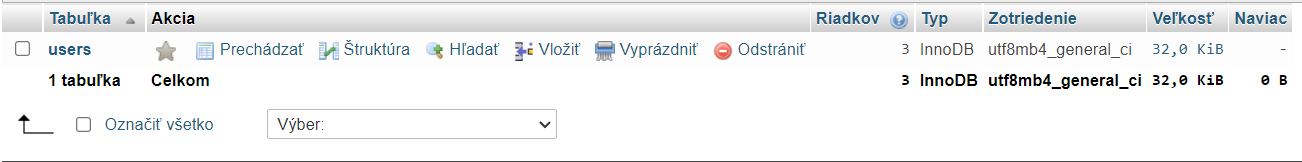
\includegraphics[width=\textwidth]{obr/tabprihlas.png}}
\caption{Vzhľad databázy pre ukladanie mien a hesiel adminov}\label{OBRAZOK 1.16}
\end{figure}


\subsection{databáza pre potreby textov a fotografií\ref{OBRAZOK 1.17}}
\vspace{0.5cm}
\textbf{Databáza pre zaradovanie textov do kategórií.}
\vspace{0.5cm}
\begin{lstlisting}
 CREATE TABLE `categories` (
  `id` int(3) NOT NULL,
  `name` text NOT NULL
) ENGINE=InnoDB
\end{lstlisting}

\vspace{0.5cm}
\textbf{Databáza pre uskladnenie a prácu s textami.}
\vspace{0.5cm}
\begin{lstlisting}
CREATE TABLE `posts` (
  `id` int(6) NOT NULL,
  `cat_id` int(3) NOT NULL,
  `title` varchar(255) CHARACTER SET utf8 COLLATE utf8_bin NOT NULL,
  `contents` text CHARACTER SET utf8 COLLATE utf8_bin NOT NULL,
  `date_posted` datetime NOT NULL
) ENGINE=InnoDB DEFAULT CHARSET=utf8;
\end{lstlisting}

\vspace{0.5cm}
\textbf{Databáza pre uskladnenie a prácu s fotografiami.}
\vspace{0.5cm}
\begin{lstlisting}
CREATE TABLE `images` (
  `id` int(11) NOT NULL,
  `title` text CHARACTER SET utf8 COLLATE utf8_bin NOT NULL,
  `description` text CHARACTER SET utf8 COLLATE utf8_bin NOT NULL,
  `filepath` text NOT NULL,
  `uploaded_date` datetime NOT NULL DEFAULT current_timestamp()
) ENGINE=InnoDB DEFAULT CHARSET=utf8;
\end{lstlisting}


\begin{figure}[!tbh]
\centering
\setlength{\fboxsep}{0pt}%
\setlength{\fboxrule}{1pt}%
\fbox{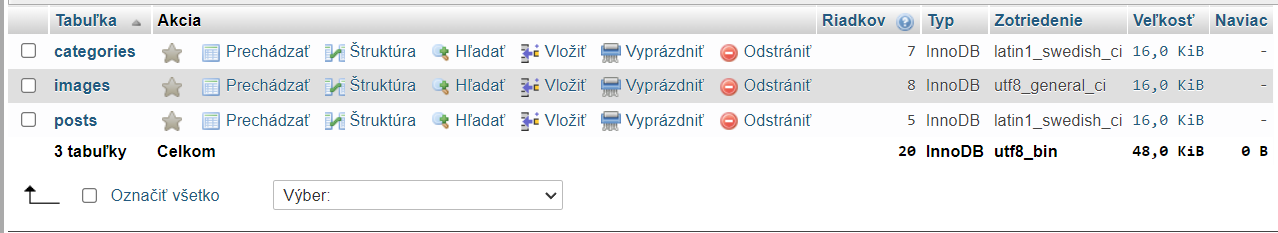
\includegraphics[width=\textwidth]{obr/tabblog.png}}
\caption{Vzhľad databázi pre potreby textov a fotografií}\label{OBRAZOK 1.17}
\end{figure}
